\chapter{Tri rapide}
\section {Description}
Le tri rapide, aussi appelé "tri de Hoare" du nom de son inventeur "Tony Hoare" ou "Quick Sort" en anglais, est considéré comme l'algorithme le plus performant des tris en table qui est certainement celui qui est le plus employé dans les programmes depuis son invention en 1960. Cette méthode illustre le principe dit « diviser pour régner », qui consiste à appliquer récursivement une méthode destinée à un problème de taille donnée à des sous-problèmes similaires, mais de taille inférieure. Ce principe général produit des algorithmes qui permettent souvent d’importantes réductions de complexité

\section{Fonctionnement de l'algorithme}
Le principe de ce tri est d’ordonner le vecteur T[n] en cherchant dans celui-ci une clé pivot autour de laquelle réorganiser ses éléments. Donc On considère un élément au hasard dans le tableau, le pivot et on procède à une partition du tableau en 2 zones : les éléments inférieurs ou égaux au pivot dans un coté et les éléments supérieurs ou égaux au pivot
dans l'autre coté pui on place le pivot dans sa position appropriée. On répète récursivement la procédure sur chacune des partitions créées en considérant un pivot dans chaque partie jusqu’à ce qu’elle soit réduite à une liste à un seul élément. [3]
\begin{figure} [H]
        \centering
        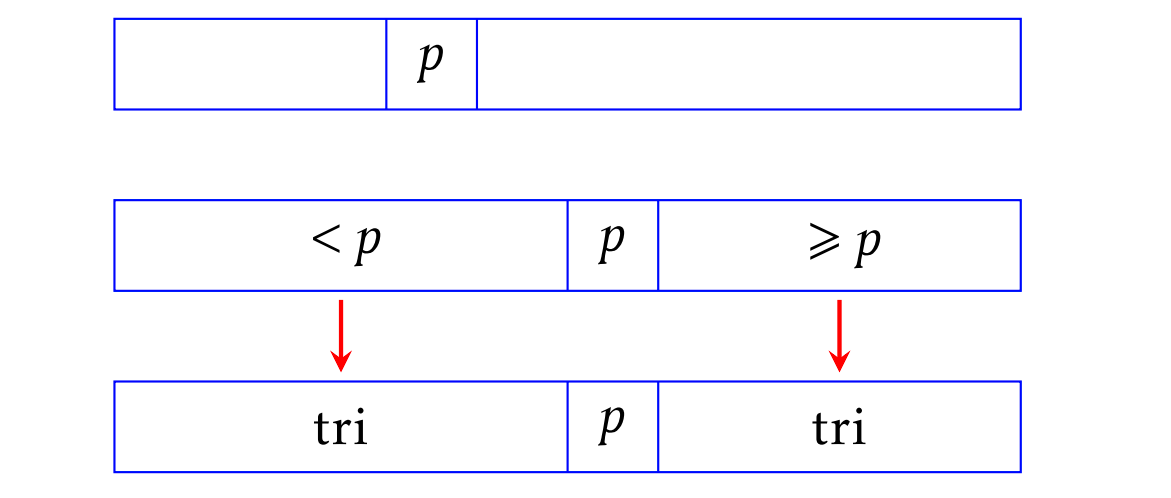
\includegraphics[scale=0.4]{ressources/tri_rapide.PNG}
        \caption{Illustration Tri Rapide }
        \label{fig:rapide}
     \end{figure}
Ils existent plusieurs methodes de choix du pivot qui est determinant pour la performance de l'algorithme:
\begin{enumerate}
    \item Le pivot est le premier élément du tableau
    \item Le pivot est le dernier élément du tableau
    \item Le pivot est au millieu du tableau
    \item Le pivot est choisi au hasard
    \item pivot est trouvé en recherchant la médiane
\end{enumerate}
Dans ce TP nous avons testé les trois premières méthodes comme il est demandé dans l'énoncé.\\
Pour programmer le Tri Rapide nous allons utiliser deux procédures:
\begin{enumerate}
    \item Partition:une fonction qui divise un tableau en entrée en deux sous listes et retourne le pivot. Il peut y avoir plusieurs façons de faire la partition, dans le cas de la première et la deuxième methodes  on commençe le parcours du tableau par l'élément le plus à gauche ou à droite selon le pivot choisi et on utilise un compteur p qui garde la trace de l'indice des éléments plus grands que le pivot. Pendant le parcours, si on trouves un élément plus petit que le pivot, on incrémente p et l'élément actuel sera échangé avec Tab[p]. Sinon il sera ignoré.
    Dans la troisième méthode on parcourt le tableaux à partir des deux extrémités, jusqu'à rencontrer un élément supérieur au pivot dans la prtie droite du tableau ou le contraire dans la pertie gauche et on permute entre les deux.
\end{enumerate}
Partition  ainsi que la procédure TriRapide qui assure l'application du 
même processus sur les sous listes droites et gauches générées (assure la récursivité).\\
\subsection{Méthode 1 : Le pivot est le premier élément du tableau }
\par
\begin{function}[H]
    \textbf{Variables :}\\
     i : entier\;
     p,pivot : entier\;
    \Begin{
        $p \leftarrow deb$\;
        $pivot \leftarrow tab[deb]$\;
        \For{$i \leftarrow deb+1$ \KwTo fin$}{
            \If {tab[i]$<pivot$} {
                p++ \;
                permuter(tab[i]$,p$);
            }
        }
        permuter(tab[p]$,deb$)\;
        \textbf {retourner} p;
      
    }
    \caption{Partition1(Entrée: tab: tableau d'entier, deb:entier, fin:entier)}
\end{function}

\par
\begin{function}[H]
    \textbf{Variables :}\\
     pivot : entier\;
    \Begin{
            \If {deb$<fin$} {
                pivot$ \leftarrow Partition1(tab$,deb$,fin$) \;
                TriRapide1$(tab$, deb$, pivot-1$) \;
                TriRapide1$(tab$, pivot+1$,fin$) \;
                
            }
         }
    \caption{TriRapide1(Entrée: tab: tableau d'entier, deb:entier, fin:entier)}
\end{function}

\subsection{Méthode 2 : Le pivot est le dernier élément du tableau}
\par
\begin{function}[H]
    \textbf{Variables :}\\
     i : entier\;
     p,pivot : entier\;
    \Begin{
        $p \leftarrow fin$\;
        $pivot \leftarrow tab[fin]$\;
        \For{$i \leftarrow fin-1$ \KwTo deb$}{
            \If {tab[i]$ > pivot$} {
                p-- \;
                permuter(tab[i]$,p$);
            }
        }
        permuter(tab[p]$,fin$)\;
        \textbf {retourner} p \;
      
    }
    \caption{Partition2(Entrée: tab: tableau d'entier, deb:entier, fin:entier)}
\end{function}
\par
\begin{function}[H]
    \textbf{Variables :}\\
     pivot : entier\;
    \Begin{
            \If {deb$<fin$} {
                pivot$ \leftarrow Partition2(tab$,deb$,fin$) \;
                TriRapide2$(tab$, deb$, pivot-1$) \;
                TriRapide2$(tab$, pivot+1$,fin$) \;
                
            }
         }
    \caption{TriRapide2(Entrée: tab: tableau d'entier, deb:entier, fin:entier)}
\end{function}
\subsection{Méthode 3 : Le pivot est au millieu du tableau}
\par
\begin{function}[H]
    \textbf{Variables :}\\
     i,j,x: entier\;
     pivot: entier\;
    \Begin{
        $x \leftarrow (fin$-deb$)/2$ \;
        $pivot \leftarrow $tab[x] \;
        $i \leftarrow deb-1$ \;
        $j\leftarrow fin$\;
        \While {i<=j}
        {
           \While {$tab[i]<pivot$;} {$i \leftarrow $i+1 ;}
           \While  {$tab[j]>pivot$;} {$j \leftarrow $j+1 ;}
           \If{i$<=j$}{$Permuter($tab,$i,$j);}
           }
        
    \textbf{retourner} $i\;\\
     }
    \caption{Partition3(Entrée: tab: tableau d'entier, deb:entier, fin:entier)}
\end{function}

\par
\begin{function}[H]
    \textbf{Variables :}\\
     pivot : entier\;
    \Begin{
            \If {deb$<fin$} {
                pivot$ \leftarrow Partition3(tab$,deb$,fin$) \;
                TriRapide3$(tab$, deb$, pivot-1$) \;
                TriRapide3$(tab$, pivot+1$,fin$) \;
                
            }
         }
    \caption{TriRapide3(Entrée: tab: tableau d'entier, deb:entier, fin:entier)}
\end{function}
\section{Calcul de complexité}
\subsection{Complexité temporelle}
Pour calculer la complexité des algorithmes récursives de Tri Rapide nous utilisons la formule suivante : \\
le nombre des niveaux de partition * temps nécessaire pour un niveau

sachant que la complexité temporelle pour réaliser la partition  est de l'ordre O(n) car à chaque niveau de partitionnement,un total de n éléments sera divisé en partitions gauche et droite (1 × n au premier niveau, 2 × n/2 au deuxième, 4 × n/4 au troisième, etc.) L'effort total est donc le même à tous les niveaux de partitionnement.\\


   \begin{enumerate}
    \item Meilleur cas: le meilleur ca s'achève lorsque le tableau Tab de taille n se divise sur 2 partie égales de n/2 éléments et les sous tableaux a leurs tour se divisent en deux sous-listes de même taille.
      \begin{figure} [H]
        \centering
        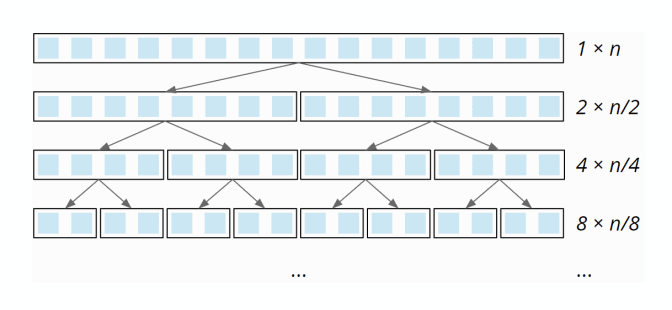
\includegraphics[scale=0.45]{ressources/Quicksort_best_case_time_complexity.png}
        \caption{Tri Rapide complexité meilleur cas }
        \label{fig:rapide}
     \end{figure}
     
    Le nombre des niveaux de partition:
    \[
   \frac{n}{2^k}=1
   \]
    \[
   n=2^k
   \]
    \[
   \log_2 n = k \log_2 2
   \]
  \[
   k= \log_2 n
  \]
  Donc Dans le meilleur des cas, la complexité temporelle est : O(n * log n)\\
  Cette complexité est atteinte dans le cas suivant:\\
    *le pivot choisi est le premier élément dans le tableau ou le dernier et les éléments sont aléatoires.\\
    * le pivot choisi est toujours au millieu du tableau
     
   \item Pire cas: le pire cas correspond au cas où le tableau ne serait pas divisé en deux partitions de tailles approximativement égales, mais une de longueur 0 et une de longueur n-1 (tous les éléments sauf l'élément pivot) alors l'effort de partitionnement décroît linéairement de n à 0 avec la liste droite ou gauche vide selon le pivot choisi.
   Ainsi nous calculons la comlexité comme suit: 
   \[
   n+n-2+n-3+n-4...+2 =\frac{n(n+1)}{2}-1 \\
   = n^2 + n \\
   = O(n^2) \\
   \]
   \begin{figure} [H]
       \centering
       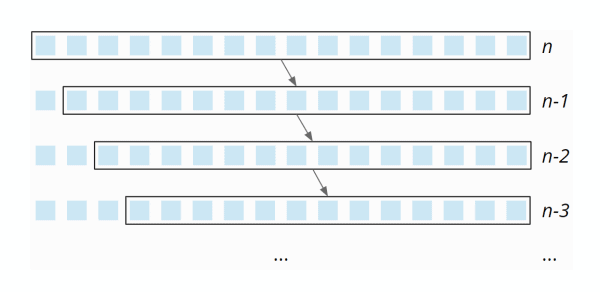
\includegraphics[scale=0.45]{ressources/Quicksort_worst_case_time_complexity-600x292.png}
       \caption{Tri Rapide complexité pire cas}
       \label{fig:rapidel}
   \end{figure}
    Cette complexité est atteinte lorsque le pivot choisi est a la tête ou a la fin du tableau et ce dernier est triée d'une manière descendante ou ascendante.
   \item Moyen cas: est atteint lorsque le tableau serait divisé successivement
en deux sous-listes de taille à peu près équivalente par exemple n/10 et 9n/10.
En utilisons la formule au dessus nous aboutissons à une complexité similaire au meilleur cas O(n * log n).
\end{enumerate}

  


\subsection{Complexité spatiale}
La complexité spatiale de Tri Rapide est dans tout les cas O(log n)
car pour chaque niveau de récursion, nous avons besoin de mémoire supplémentaire sur la pile. Come nous avons vu quand nous avons calculé la complexité temporelle dans le cas moyen et le meilleur cas, la profondeur maximale de récursion est limitée par O(log n) .
Dans le pire des cas, la profondeur maximale de récursion est de n
\section{Experimentation}
Dans cette partie nous allons voir les résultats des exécutions des trois méthodes de l'algorithme de Tri Rapide sur différentes taille de tableau qui se représentent en 3 configuration ( triée en bon ordre , triée en ordre inverse , aléatoire) 
\subsection{Les données de tableau sont triées en bon ordre}

 \begin{figure}[H]
    \centering
        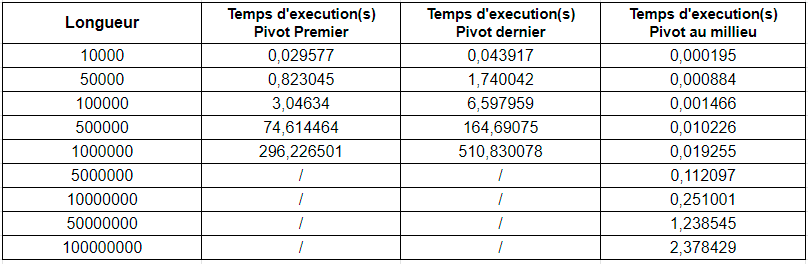
\includegraphics[scale=0.7]{ressources/trieeT.PNG}
        \caption{Tableau représentant le temps d'execution en s des trois méthodes de tri rapide selon les différentes tailles des données d'entrée triées en bon ordre}
    \label{fig:fusion}
\end{figure}
\par
 \begin{figure}[H]
    \centering
        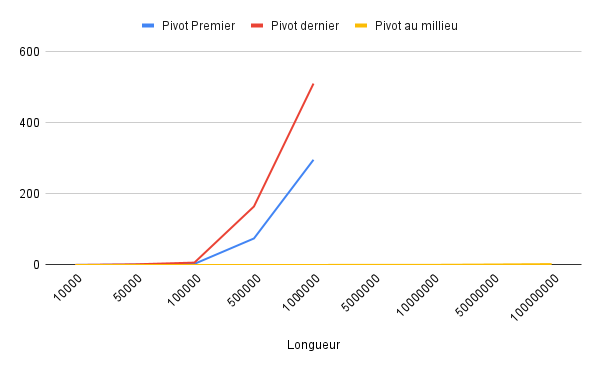
\includegraphics[scale=0.7]{ressources/triee.png}
        \caption{graphique représentant le temps d'execution en s des trois méthodes de tri rapide selon les différentes tailles de tableau}
    \label{fig:fusion}
\end{figure}


\subsection{Les données de tableau sont triées en ordre inverse }
\begin{figure}[H]
    \centering
        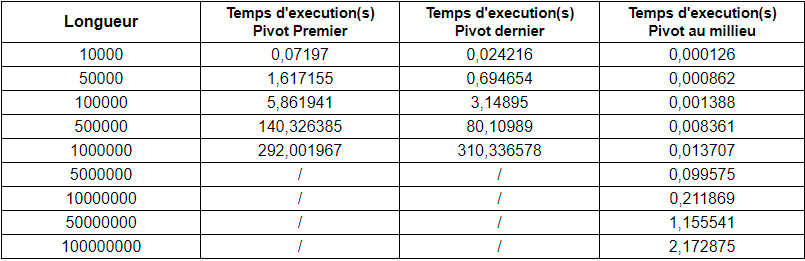
\includegraphics[scale=0.7]{ressources/invT.PNG}
        \caption{Tableau représentant le temps d'execution en s des trois méthodes de tri rapide selon les différentes tailles des données d'entrée triées en ordre inverse}
    \label{fig:fusion}
\end{figure}

\begin{figure}[H]
    \centering
        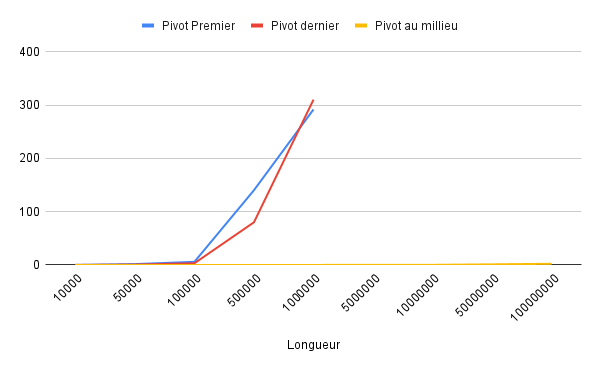
\includegraphics[scale=0.7]{ressources/inv.png}
        \caption{graphique représentant le temps d'execution en s des trois méthodes de tri rapide selon les différentes tailles de tableau}
    \label{fig:fusion}
\end{figure}

\subsection{Les données de tableau sont positionnés aléatoirement}
\begin{figure}[H]
    \centering
        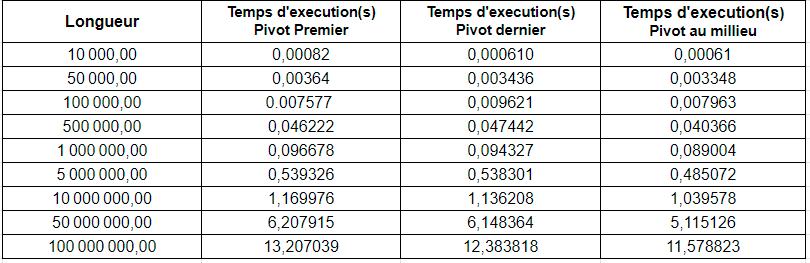
\includegraphics[scale=0.7]{ressources/randT.PNG}
        \caption{Tableau représentant le temps d'execution en s des trois méthodes de tri rapide selon les différentes tailles des données d'entrée sont aléatoires}
    \label{fig:fusion}
\end{figure}

\begin{figure}[H]
    \centering
        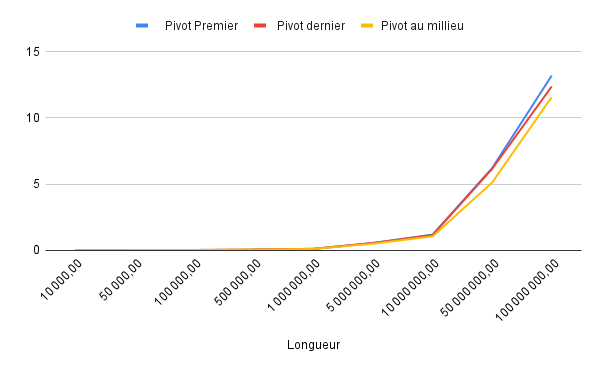
\includegraphics[scale=0.7]{ressources/random.png}
        \caption{graphique représentant le temps d'execution en s des trois méthodes de tri rapide selon les différentes tailles de tableau}
    \label{fig:fusion}
\end{figure}
\section{Analyses Des Résultats}
\paragraph{Cas Pivot au début:} \\
Pour des données d'entrée distribuées de manière aléatoire, le temps nécessaire est légèrement supérieur au double si la taille du tableau est doublée. Cela correspond au temps d'exécution quasi-linéaire attendu O(n log n).\\
Pour les données d'entrée triées dans l'ordre croissant ou décroissant, le temps requis quadruple lorsque la taille de l'entrée est doublée, nous avons donc un temps quadratique O(n²).\\
Le tri des données dans l'ordre décroissant ne prend qu'un peu plus de temps que le tri des données dans l'ordre croissant et l'execution s'arrete si la taille de tableau dépasse 10^6.
\paragraph{Cas Pivot au dérnier:} 
Dans ce cas de choix de pivot les résultas sont approximativement similaires aux ceux de choix de pivot au début: une complexité O(n log n) pour des données de tableau  aléatoires et O(n²) si les données sont triées avec une légère amélioration sur les tableaux triées dans l'ordre décroissant.\\
\paragraph{cas Pivot au millieu :}
Pour des données d'entrée triées et non triées l'étude de l'évolution de temps d'execution correspond au temps d'exécution quasi-linéaire attendu O(n log n).\\
L'algorithme est nettement plus rapide pour les données d'entrée prétriées que pour les données aléatoires.\\

\section{Conclusion}
Le Tri rapide est l’algorithme de tri le plus utilisé en raison de sa complexité temporelle optimale en moyenne de O(n log n) et sa complexité spatiale O(log n) ce qui en fait un excellent choix pour les situations où l'espace est limité. 
Bien qu'il offre ces avantages il est considéré comme instable à cause des permutations des éléments et très improbable avec choix du pivot qui affecte considérablement sa complexité où elle atteint O(n^2)$ dans les pires cas mais il reste le meilleur choix partout où la stabilité n'est pas nécessaire.
